\documentclass[12pt,a4paper,openany]{ctexbook}

% ========== 宏包 ==========
\usepackage[margin=2.5cm]{geometry}
\usepackage{listings}
\usepackage{xcolor}
\usepackage{hyperref}
\usepackage{enumitem}
\usepackage{booktabs}
\usepackage{fancyhdr}
\usepackage{tcolorbox}
\usepackage{titlesec}

\usepackage{graphicx}
\graphicspath{{Images/}} 

% ========== 代码样式 ==========
\definecolor{codebg}{RGB}{248,248,248}
\definecolor{codeframe}{RGB}{200,200,200}
\definecolor{cmtgreen}{RGB}{0,128,0}
\definecolor{kwblue}{RGB}{0,0,180}
\definecolor{strred}{RGB}{180,0,0}

\lstdefinestyle{mininetstyle}{
	backgroundcolor=\color{codebg},
	frame=single,
	rulecolor=\color{codeframe},
	basicstyle=\ttfamily\small,
	keywordstyle=\color{kwblue}\bfseries,
	commentstyle=\color{cmtgreen}\itshape,
	stringstyle=\color{strred},
	breaklines=true,
	showstringspaces=false,
	tabsize=4,
	language=Python,
	morekeywords={sudo,mn,pingall,iperf,ovs-ofctl,ifconfig,exit,help,net,links,dump}
}

\lstdefinestyle{bashstyle}{
	backgroundcolor=\color{codebg},
	frame=single,
	rulecolor=\color{codeframe},
	basicstyle=\ttfamily\small,
	keywordstyle=\color{kwblue}\bfseries,
	commentstyle=\color{cmtgreen}\itshape,
	breaklines=true,
	showstringspaces=false,
	language=bash,
}

% ========== 页眉页脚 ==========
\pagestyle{fancy}
\fancyhf{}
\fancyhead[LE,RO]{\thepage}
\fancyhead[LO]{\rightmark}
\fancyhead[RE]{\leftmark}
\renewcommand{\headrulewidth}{0.4pt}
\fancypagestyle{plain}{
	\fancyhf{}
	\fancyhead[LE,RO]{\thepage}
	\renewcommand{\headrulewidth}{0pt}
}

% ========== 章节标题样式 ==========
\titleformat{\chapter}[hang]
{\normalfont\huge\bfseries}
{\thechapter}{1em}{}
\titlespacing*{\chapter}{0pt}{-20pt}{20pt}

% ========== 目录深度 ==========
\setcounter{tocdepth}{2}
\setcounter{secnumdepth}{2}

% ========== 超链接 ==========
\hypersetup{
	colorlinks=true,
	linkcolor=blue,
	urlcolor=blue,
	citecolor=blue,
	bookmarksnumbered=true,
}

% ========== 自定义盒子 ==========
\newtcolorbox{tipbox}{
	colback=blue!5,
	colframe=blue!40,
	title=提示,
	fonttitle=\bfseries,
}

\newtcolorbox{warnbox}{
	colback=red!5,
	colframe=red!40,
	title=注意,
	fonttitle=\bfseries,
}

% ========== 标题信息 ==========
\title{\textbf{Mininet}}
\author{WangFei}
\date{2026/10/28}

\begin{document}

% ========== 封面 ==========
\frontmatter
\maketitle

% ========== 前言 ==========
\chapter{前言}
本教程面向希望系统掌握 Mininet 的读者，从环境搭建到 Python API 编程，再到与 SDN 控制器集成，逐步深入。每章配有可运行的命令与脚本示例，建议边读边在实验环境中验证。

\tableofcontents

% ========== 正文 ==========
\mainmatter

\part{基础篇}

% ============================================================
\chapter{引言：什么是 Mininet}
% ============================================================

\section{Mininet 的定义}

Mininet 是一个轻量级的网络仿真器，能够在单台机器上创建一个包含虚拟主机、交换机、链路和控制器的完整网络。它利用 Linux 的网络命名空间（network namespace）实现进程级虚拟化，每个虚拟主机表现为一个拥有独立网络接口的 \texttt{bash} 进程。

\section{为什么学习 Mininet}

Mininet 在软件定义网络（SDN）的学习与研究中被广泛使用，主要原因包括：

\begin{itemize}[leftmargin=*]
	\item \textbf{快速原型验证}：一条命令即可创建包含数十个节点的网络，数秒内完成启动。
	\item \textbf{真实协议栈}：虚拟主机运行真实的 Linux 网络栈，可运行 \texttt{ping}、\texttt{iperf}、\texttt{wget} 等任意标准工具。
	\item \textbf{OpenFlow 支持}：与 Open vSwitch 和各类 SDN 控制器无缝集成，便于开发控制平面应用。
	\item \textbf{可迁移性}：在 Mininet 上验证的拓扑和控制器逻辑，可较为顺利地移植到真实硬件。
\end{itemize}

\section{学习路径概览}

本教程按以下顺序组织：
\begin{enumerate}[leftmargin=*]
	\item 环境搭建与安装
	\item 基础命令与 CLI 交互
	\item 内置拓扑与自定义拓扑
	\item Python API 编程
	\item 链路参数与性能测试
	\item 与 SDN 控制器的集成
	\item 综合实验与调试技巧
\end{enumerate}


% ============================================================
\chapter{环境搭建与安装}
% ============================================================

\section{安装方式选择}

Mininet 官方支持三种主要安装方式，各有适用场景：

\begin{center}
	\begin{tabular}{@{}p{2.6cm}p{3.2cm}p{3.2cm}p{3.4cm}p{1cm}@{}}
		\toprule
		\textbf{方式} & \textbf{适用场景} & \textbf{优点} & \textbf{缺点} & \textbf{难度} \\
		\midrule
		预打包虚拟机 & 初学者、非 Linux 主机、快速上手 & 开箱即用，不污染宿主机 & 额外虚拟化开销 & 低 \\
		Ubuntu 包安装 & 日常开发、快速部署、无虚拟机开销 & 一条命令完成，干净 & 版本可能较旧，不一定支持 Python 3 & 中 \\
		源码安装 & 需要最新版或自定义组件 & 灵活，可控制组件与版本 & 步骤多，脚本可能改动系统 & 高 \\
		\bottomrule
	\end{tabular}
\end{center}

官方推荐初学者从 VM 镜像开始，因为这是“最万无一失”的方式\footnote{参见 Mininet 官方文档 \url{http://mininet.org/download/}}。

\section{方式一：预打包虚拟机（推荐初学者）}

Mininet 官方提供预配置的 Ubuntu 虚拟机镜像，已预装 Mininet、OpenFlow 工具及相关内核调整，支持 VMware、VirtualBox、QEMU/KVM 等主流虚拟化平台。

\subsection{操作步骤}

\begin{enumerate}[leftmargin=*]
	\item 从 Mininet Releases 页面下载 VM 镜像（通常为 OVF 格式，压缩后约 1 GB）。
	\item 在 VirtualBox 或 VMware 中导入该 OVF 文件。
	\item 启动虚拟机，使用默认凭据登录（通常为 \texttt{mininet/mininet}）。
	\item 在终端执行 \texttt{sudo mn --test pingall} 验证环境。
\end{enumerate}

\begin{tipbox}
	VM 方式的最大优势是不影响宿主机已有环境。如果宿主机是多用户系统，或你不希望在日常使用的机器上直接改动网络配置，VM 是最稳妥的选择。
\end{tipbox}

\section{方式二：Ubuntu 包管理器安装}

适用于 Ubuntu 16.04 及以上版本，安装 Mininet 核心及 Python API：

\begin{lstlisting}[style=bashstyle]
	sudo apt-get update
	sudo apt-get install mininet
\end{lstlisting}

安装后执行 \texttt{mn --version} 确认版本。

\begin{warnbox}
	包管理器中的 Mininet 版本可能较旧，且不一定支持 Python 3。如果需要最新功能或 Python 3 支持，应选择源码安装。
\end{warnbox}

\section{方式三：源码安装（最新版本/自定义）}

源码安装通过项目自带的 \texttt{util/install.sh} 脚本完成，支持 Ubuntu、Debian 和 Fedora。这是获取最新 Mininet 版本的推荐方式。

\subsection{基本步骤}

\begin{lstlisting}[style=bashstyle]
	# 1. 安装基础依赖
	sudo apt update
	sudo apt install git build-essential -y
	
	# 2. 克隆源码
	git clone https://github.com/mininet/mininet.git
	cd mininet
	
	# 3. 可选：切换到指定版本
	git tag                    # 列出可用版本
	git checkout 2.3.0         # 以 2.3.0 为例
	
	# 4. 运行安装脚本
	sudo ./util/install.sh -a  # 完整安装
\end{lstlisting}

\texttt{install.sh} 的常用选项包括：

\begin{center}
	\begin{tabular}{@{}ll@{}}
		\toprule
		\textbf{选项} & \textbf{说明} \\
		\midrule
		\texttt{-a} & 安装全部组件（Mininet、OVS、控制器、Wireshark 插件等） \\
		\texttt{-nV} & 仅安装 Mininet 和 Open vSwitch \\
		\texttt{-nfv} & 安装 Mininet、OpenFlow 参考实现和 OVS \\
		\texttt{-s <dir>} & 将源码安装到指定目录而非 home \\
		\bottomrule
	\end{tabular}
\end{center}

\subsection{重要警告}

官方 INSTALL 文件明确提示：\texttt{install.sh} 可能“具有侵入性”，会在 home 目录下创建 \texttt{mininet}、\texttt{openflow}、\texttt{oftest}、\texttt{pox} 等多个目录，\textbf{有可能损坏现有系统或 home 目录}。因此：

\begin{itemize}[leftmargin=*]
	\item 建议先在 VM 或测试机中尝试，确认无误后再用于日常工作机。
	\item 运行前备份重要数据。
	\item 可先阅读 \texttt{util/install.sh} 内容，了解具体改动。
\end{itemize}

如果只需要最小可用的 Mininet + OVS，使用 \texttt{./util/install.sh -nv} 相对温和，不会安装额外控制器和工具。

\section{安装后清理}

无论采用哪种方式，每次运行 Mininet 后建议执行：

\begin{lstlisting}[style=bashstyle]
	sudo mn -c
\end{lstlisting}

该命令清理残留的虚拟接口和进程，避免下次启动时报 “address already in use” 等错误。

% ============================================================
\chapter{基础命令与 CLI 交互}
% ============================================================

\section{第一条 Mininet 命令}

最简单的启动方式是不带任何参数：

\begin{lstlisting}[style=bashstyle]
	sudo mn
\end{lstlisting}

该命令会创建如图 \ref{fig:default_topo} 所示的默认拓扑：包含 1 台交换机 \texttt{s1}、2 台主机 \texttt{h1} 和 \texttt{h2}，以及 1 台控制器 \texttt{c0}。进入 CLI 后提示符变为 \texttt{mininet>}。图中的蓝色实线代表数据平面的以太网链路，红色虚线代表交换机与控制器之间的 OpenFlow 控制链路。

\begin{figure}[htbp]
	\centering
	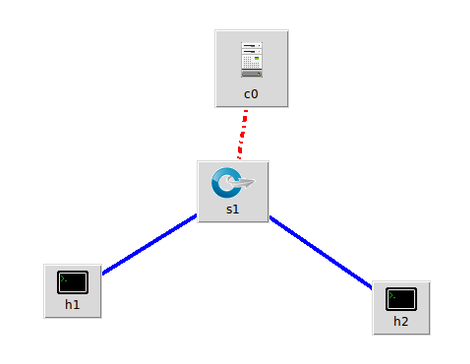
\includegraphics[width=0.6\textwidth]{Images/default_topology.png}
	\caption{Mininet 默认拓扑结构}
	\label{fig:default_topo}
\end{figure}

\section{CLI 核心命令}

进入 CLI 后，可以使用两类命令：Mininet 内置命令和节点命令。

\subsection{Mininet 内置命令}

\begin{center}
	\begin{tabular}{@{}ll@{}}
		\toprule
		\textbf{命令} & \textbf{功能} \\
		\midrule
		\texttt{help} & 列出所有可用命令 \\
		\texttt{net} & 显示拓扑中的节点和链路 \\
		\texttt{links} & 列出所有链路 \\
		\texttt{dump} & 输出所有节点的详细信息 \\
		\texttt{pingall} & 测试所有主机两两连通性 \\
		\texttt{iperf} & 测试两台主机间的带宽 \\
		\texttt{exit} & 退出 Mininet \\
		\bottomrule
	\end{tabular}
\end{center}

\subsection{在节点上执行命令}

在 CLI 中，以节点名开头即可在该节点上执行任意 Linux 命令：

\begin{lstlisting}[style=bashstyle]
	mininet> h1 ifconfig
	mininet> h2 ping -c 3 h1
	mininet> h1 python -m http.server 80 &
\end{lstlisting}

\section{启动选项示例}

\texttt{mn} 命令支持丰富的启动参数，常用的包括：

\begin{lstlisting}[style=bashstyle]
	# 指定树形拓扑：深度2，扇出3
	sudo mn --topo tree,depth=2,fanout=3
	
	# 启动时为每个节点打开 xterm 窗口
	sudo mn -x
	
	# 指定交换机类型为 Open vSwitch
	sudo mn --switch ovs
	
	# 运行连通性测试后不进入 CLI
	sudo mn --test pingall
\end{lstlisting}


\part{进阶篇}

% ============================================================
\chapter{内置拓扑与自定义拓扑}
% ============================================================

\section{内置拓扑类型}

Mininet 提供多种参数化拓扑，可通过 \texttt{--topo} 指定：

\begin{center}
	\begin{tabular}{@{}ll@{}}
		\toprule
		\textbf{拓扑} & \textbf{参数与说明} \\
		\midrule
		\texttt{single} & 单交换机，参数 \texttt{--topo single,N}（N 台主机） \\
		\texttt{linear} & 线性链，参数 \texttt{--topo linear,N} \\
		\texttt{tree} & 树形，参数 \texttt{depth=D,fanout=F} \\
		\texttt{reversed} & 单交换机反向端口分配 \\
		\bottomrule
	\end{tabular}
\end{center}

例如，创建 4 台主机连接到 1 台交换机：

\begin{lstlisting}[style=bashstyle]
	sudo mn --topo single,4
\end{lstlisting}

\section{通过 Python 脚本自定义拓扑}

内置拓扑无法满足复杂需求时，可编写 Python 脚本定义拓扑。基本模式是继承 \texttt{Topo} 类并重写 \texttt{build()} 方法：

\begin{lstlisting}[style=mininetstyle]
	from mininet.topo import Topo
	
	class MyTopo(Topo):
	def build(self):
	# 添加两台交换机
	s1 = self.addSwitch('s1')
	s2 = self.addSwitch('s2')
	
	# 添加四台主机
	h1 = self.addHost('h1')
	h2 = self.addHost('h2')
	h3 = self.addHost('h3')
	h4 = self.addHost('h4')
	
	# 添加链路
	self.addLink(h1, s1)
	self.addLink(h2, s1)
	self.addLink(h3, s2)
	self.addLink(h4, s2)
	self.addLink(s1, s2)
	
	topos = {'mytopo': (lambda: MyTopo())}
\end{lstlisting}

保存为 \texttt{mytopo.py} 后，通过以下命令启动：

\begin{lstlisting}[style=bashstyle]
	sudo mn --custom mytopo.py --topo mytopo
\end{lstlisting}


% ============================================================
\chapter{Python API 编程}
% ============================================================

\section{核心类与对象}

Mininet 的 Python API 以 \texttt{Mininet} 类为中心，该类提供创建、启动、停止网络以及运行测试的方法。常用方法包括：

\begin{center}
	\begin{tabular}{@{}ll@{}}
		\toprule
		\textbf{方法} & \textbf{功能} \\
		\midrule
		\texttt{addHost()} / \texttt{addSwitch()} & 添加节点 \\
		\texttt{addLink()} & 添加链路 \\
		\texttt{start()} / \texttt{stop()} & 启动/停止网络 \\
		\texttt{pingAll()} & 全体连通性测试 \\
		\texttt{iperf()} & 带宽测试 \\
		\texttt{interact()} & 进入 CLI \\
		\bottomrule
	\end{tabular}
\end{center}

\section{一个完整的脚本示例}

以下脚本创建一个 3 主机、1 交换机的网络，并执行 ping 测试：

\begin{lstlisting}[style=mininetstyle]
	from mininet.net import Mininet
	from mininet.topo import SingleSwitchTopo
	from mininet.cli import CLI
	
	# 创建拓扑对象
	topo = SingleSwitchTopo(k=3)
	
	# 创建 Mininet 实例并启动
	net = Mininet(topo=topo)
	net.start()
	
	# 执行测试
	net.pingAll()
	
	# 进入交互式 CLI（可选）
	CLI(net)
	
	# 停止并清理
	net.stop()
\end{lstlisting}

\section{向节点下发命令}

在脚本中可以直接调用节点的 \texttt{cmd()} 方法执行任意命令：

\begin{lstlisting}[style=mininetstyle]
	h1 = net.get('h1')
	h2 = net.get('h2')
	result = h1.cmd('ping -c 1 %s' % h2.IP())
	print(result)
\end{lstlisting}


% ============================================================
\chapter{链路参数与性能测试}
% ============================================================

\section{链路属性配置}

Mininet 支持在创建链路时指定带宽、延迟、丢包率等参数，用于模拟真实网络条件：

\begin{lstlisting}[style=mininetstyle]
	self.addLink(h1, s1, bw=10, delay='5ms', loss=2)
\end{lstlisting}

上述代码创建一个带宽 10 Mbps、延迟 5 ms、丢包率 2\% 的链路。参数 \texttt{bw}、\texttt{delay}、\texttt{loss} 由 \texttt{TCLink} 类实现。

\section{带宽测试：iperf}

在 CLI 中直接使用 \texttt{iperf} 命令测试两台主机的 TCP 带宽：

\begin{lstlisting}[style=bashstyle]
	mininet> iperf h1 h2
\end{lstlisting}

在 Python 脚本中调用：

\begin{lstlisting}[style=mininetstyle]
	net.iperf(hosts=[h1, h2], l4Type='TCP', seconds=5)
\end{lstlisting}

\section{连通性测试}

\texttt{pingAll()} 对所有主机对执行 ping 测试，返回丢包统计。在 CLI 中对应 \texttt{pingall} 命令。


\part{实战篇}

% ============================================================
\chapter{与 SDN 控制器集成}
% ============================================================

\section{控制器类型}

Mininet 支持多种控制器配置方式：

\begin{itemize}[leftmargin=*]
	\item \textbf{默认控制器}：\texttt{mn} 启动时自动运行的简单控制器 \texttt{c0}，功能有限。
	\item \textbf{RemoteController}：连接外部已运行的控制器（如 Ryu、ONOS、POX）。
	\item \textbf{内置控制器类}：如 \texttt{Ryu}、\texttt{OVSController} 等。
\end{itemize}

\section{连接外部控制器}

以 Ryu 为例，先在另一个终端启动 Ryu：

\begin{lstlisting}[style=bashstyle]
	ryu-manager ryu.app.simple_switch_13
\end{lstlisting}

然后启动 Mininet 并指定远程控制器地址：

\begin{lstlisting}[style=bashstyle]
	sudo mn --controller remote,ip=127.0.0.1,port=6633
\end{lstlisting}

\section{查看流表}

在 Mininet 运行期间，可通过 \texttt{ovs-ofctl} 查看 Open vSwitch 的流表：

\begin{lstlisting}[style=bashstyle]
	mininet> sh ovs-ofctl dump-flows s1
\end{lstlisting}

或在交换机 xterm 中执行：

\begin{lstlisting}[style=bashstyle]
	ovs-ofctl dump-flows tcp:127.0.0.1:6654
\end{lstlisting}

端口号取决于 Mininet 启动时的配置。


% ============================================================
\chapter{调试与常见问题}
% ============================================================

\section{常用调试手段}

\begin{itemize}[leftmargin=*]
	\item \textbf{xterm}：启动时加 \texttt{-x} 为每个节点打开终端，便于观察节点状态。
	\item \textbf{详细模式}：\texttt{sudo mn -v output} 打印启动过程的详细信息。
	\item \textbf{节点命令}：在 CLI 中用 \texttt{h1 ifconfig}、\texttt{h1 route -n} 检查网络配置。
	\item \textbf{流表检查}：用 \texttt{dpctl} 或 \texttt{ovs-ofctl} 确认交换机行为。
\end{itemize}

\section{常见问题与处理}

\begin{center}
	\begin{tabular}{@{}p{5cm}p{8cm}@{}}
		\toprule
		\textbf{现象} & \textbf{处理方式} \\
		\midrule
		启动时报错 “address already in use” & 执行 \texttt{sudo mn -c} 清理残留 \\
		ping 不通 & 检查控制器是否运行、流表是否下发 \\
		CLI 中命令无响应 & 确认节点名拼写正确，或先用 \texttt{net} 查看节点列表 \\
		脚本中 import 报错 & 确认 Mininet 已正确安装，Python 版本匹配 \\
		\bottomrule
	\end{tabular}
\end{center}

\begin{warnbox}
	Mininet 涉及网络命名空间的创建与删除，必须以 \texttt{sudo} 权限运行。但需注意：以 \texttt{sudo} 运行的 Python 脚本使用的是系统级 Python 环境，可能与用户环境中的包不一致。
\end{warnbox}

\subsection{常见问题：pingall 报错 command not found}

在运行 \texttt{pingall} 时，如果输出类似于：
\begin{lstlisting}[style=bashstyle]
	h1 -> *** Error: could not parse ping output: bash: ping: command not found
	X
	h2 -> *** Error: could not parse ping output: bash: ping: command not found
	X
	*** Results: 100% dropped (0/2 received)
\end{lstlisting}

这通常是因为 Mininet 的虚拟主机内部缺少 \texttt{ping} 工具。Mininet 的虚拟主机运行真实的 Linux 网络栈，但不负责预装所有基础网络工具。如果宿主机是最小化安装的系统（如精简版 Docker 镜像或服务器版 Linux），可能默认未包含 \texttt{iputils-ping} 包。

\subsubsection{解决步骤}

\textbf{第一步：在宿主机安装 ping}

退出 Mininet 命令行（输入 \texttt{exit}），在宿主机终端执行：

\begin{lstlisting}[style=bashstyle]
	# Ubuntu / Debian 系统
	apt update
	apt install -y iputils-ping
	
	# CentOS / RHEL / Fedora 系统
	dnf install -y iputils
\end{lstlisting}

\textbf{第二步：清理并重启 Mininet}

安装完成后，执行清理并重新启动：

\begin{lstlisting}[style=bashstyle]
	mn -c
	mn
\end{lstlisting}

再次运行 \texttt{pingall} 应能正常显示连通性测试结果。

\begin{tipbox}
	若安装后仍报错，可检查虚拟主机内的环境变量路径。在 Mininet CLI 中执行 \texttt{h1 which ping} 确认命令路径；若未找到，可尝试使用完整路径 \texttt{h1 /bin/ping -c 3 h2} 进行测试。
\end{tipbox}

% ============================================================
\chapter{综合实验建议}
% ============================================================

\section{实验一：对比不同交换机类型的性能}

使用 \texttt{--switch} 参数分别以 \texttt{ovsk}、\texttt{user}、\texttt{lxbr} 启动同一拓扑，运行 \texttt{iperf} 对比带宽差异。参考命令：

\begin{lstlisting}[style=bashstyle]
	sudo mn --switch ovsk --test iperf
	sudo mn --switch user --test iperf
\end{lstlisting}

用户态交换机的带宽通常显著低于内核态交换机，因为存在额外的内核—用户空间数据拷贝开销。

\section{实验二：自定义拓扑与链路限制}

编写脚本创建一个包含两台交换机的线性拓扑，在交换机间链路上设置带宽限制和延迟，然后测试端到端吞吐量和 RTT。

\section{实验三：接入外部控制器}

使用 Ryu 的 \texttt{simple\_switch\_13} 作为远程控制器，启动一个包含 4 台主机的拓扑，观察控制器日志中的 PacketIn 消息，并在 CLI 中用 \texttt{dpctl} 查看流表建立过程。


% ========== 附录 ==========
\appendix
\chapter{参考资料}

\begin{enumerate}[leftmargin=*]
	\item Mininet 官方文档：\url{http://mininet.org/}
	\item Mininet Walkthrough：\url{http://mininet.org/walkthrough/}
	\item Mininet Python API 参考：\url{http://mininet.org/api/}
	\item Mininet GitHub 仓库：\url{https://github.com/mininet/mininet}
\end{enumerate}

\end{document}